\documentclass[11pt, letterpaper]{article}
\usepackage[T1]{fontenc}
\usepackage{lmodern}
\usepackage[letterpaper, margin=1in]{geometry}
\usepackage{xcolor,booktabs,tabularx,enumitem,microtype,amsmath,array}
\usepackage[font=small,labelfont=bf]{caption}
\usepackage{float}
\usepackage{tikz,pgfplots}
\pgfplotsset{compat=1.18}
\usetikzlibrary{positioning,arrows.meta}
\usepackage[hidelinks]{hyperref}

\definecolor{heading}{RGB}{47,79,111}
\definecolor{cA}{RGB}{120,144,170}
\definecolor{cB}{RGB}{200,160,90}
\definecolor{cC}{RGB}{60,110,90}
\setlist{itemsep=1pt,topsep=2pt,parsep=0pt,leftmargin=1.4em}
\newcommand{\n}{$-$}
\newcommand{\repo}{\url{https://github.com/myyquq/JevScholar}}
\newcolumntype{V}{!{\vrule}}

\title{\vspace{-2em}\bfseries Allocating a Research Budget for Scientific Synthesis:\\
A Decision-Model Controller and Draft-Guided Evidence}
\author{Final Report \quad$\cdot$\quad Group Members: Aijing Yang, Yue Ma\\[2pt]
\normalsize Code: \repo}
\date{}

\begin{document}
\maketitle
\vspace{-2em}

\begin{abstract}
\noindent
Deep research systems spend much of their inference budget deciding what to read. In our repaired
reproduction of DeepScholar-base (DS-base), screening and ranking candidate papers account for 62\%
of the cost of writing a related-work section. We ask whether a 3B decision model, d1-3B, can take
over these retrieval decisions and keep DS-base's quality at a fraction of its cost, with the
executor model, tools and search access held equal. On 180 held-out DeepScholar-Bench tasks the
controller costs 28\% of DS-base and raises claim support by 0.122, but its nugget coverage, the
share of the paper's key points that the report covers, falls by 0.053, so the registered claim
fails. Supervised and reinforcement-learning versions learn to stop after one batch and fail
validation. A diagnostic points to the writer's input: DS-base without the draft its search agent
writes loses as much coverage as the controller and gains about as much citation support. DraftRef
therefore gives DS-base's writer the papers its draft names and drops the costly relevance filter,
with d1 filling short lists. On the same test tasks it costs 41\% of DS-base, keeps nugget coverage
within a 0.02 margin and raises reference recall by 0.042. An instruction to end each sentence where
its source changes then raises citation precision from 0.399 to 0.712.
\end{abstract}

\section{Introduction}

A deep research system answers a question by searching, reading and writing. DeepScholar-Bench
\cite{patel2025deepscholar} tests the scientific case: given a paper's abstract, write its
related-work section from sources published before it. The benchmark's reference system,
DeepScholar-base (DS-base), runs a search agent, screens every candidate paper with an LLM relevance
filter, ranks the relevant ones and writes from the top 30. In our reproduction the writer costs
about 2\% of a task, while screening and ranking about 177 candidates cost 62\%. Most of the budget
goes to deciding what to read.

A small model could make that decision. We let LiquidAI's d1-3B \cite{liquidai2026d1} choose which
search to screen next and when to stop, while the executor model still proposes queries, judges
relevance and writes. d1 reads a state and a few numbered options and returns each option's
probability in one forward pass, without generating text. We also train it on its own retrieval
decisions, first with supervised labels from alternatives it actually executes and then with
reinforcement learning kept close to the supervised model \cite{shao2024deepseekmath}.

The course asks which changes to retrieval, evidence selection or synthesis most improve the
completeness and reliability of a research report. We hold the executor, tools, search access and
cost accounting equal, and we register the main claim before a held-out test: the controller must
cost less than DS-base while staying within fixed margins on coverage, citation quality and
reference recall. The claim fails. The controller costs far less and its citations are better
supported, but it covers fewer of the paper's key points, and its trained versions learn to stop
after one batch.

The controller's gap points to the writer's input rather than to its screening decisions. DS-base
hands its writer the search agent's draft, and removing the draft from DS-base produces the same
loss of coverage and a similar gain in citation support. The draft also names the papers it was
written from, yet DS-base's 30 documents keep only about half of them. DraftRef gives the writer all
of them. It stays within a 0.02 margin of DS-base's coverage at 41\% of the cost and cites more of
the important references. A change to the writer's citation instruction then raises citation
precision from 0.399 to 0.712.

Our contributions are:
\begin{enumerate}
  \item a repaired DS-base and evaluation, with two pipeline bugs and three metric defects fixed and
  DeepSeek judges checked against the official ones (Section~\ref{sec:setup});
  \item a registered, held-out test of retrieval control by d1 and its trained versions against a
  fixed rule, Simple RAG and DS-base (Sections~\ref{sec:controller} and~\ref{sec:results});
  \item a diagnosis that ties the coverage gap to what the writer receives (Section~\ref{sec:diagnosis});
  \item DraftRef and a citation rule, which keep DS-base's coverage within the margin and raise
  reference recall and citation precision at about 40\% of its cost (Section~\ref{sec:draftref}).
\end{enumerate}

\section{Task, baseline and evaluation}
\label{sec:setup}

\paragraph{Task and data.} A DeepScholar-Bench task gives a paper's abstract and publication date,
and the system writes the paper's related-work section using only papers published before it. All
systems search one frozen local arXiv index of 3.2 million papers with BM25 \cite{robertson2009bm25}
over titles and abstracts, so the evidence is abstracts. We split the June 2025 release (63 papers)
into 34 training, 9 validation and 20 development tasks, and the November 2025 release (200 papers)
into 20 development and 180 held-out test tasks. Each task lists important citations, the references
the dataset marks as essential; only evaluation and training rewards see them. DeepResearch Bench II
(DRB2) \cite{li2026drb2} serves as a six-task transfer check. ResearchQA \cite{li2025researchqa}
appears only in the baseline record (Appendix~\ref{app:benchmarks}).

\paragraph{Systems and conditions.} Every system uses the same executor, DeepSeek-V4.1-Flash
\cite{deepseek2026v41flash}, with reasoning disabled and DS-base's own sampling settings, and the
same tools, access policy and output limits; all results come from one model version. The paper used
OpenAI and Llama models, so our absolute scores differ from its scores, but every comparison here is
between systems on the same executor. Simple RAG retrieves the top 20 abstracts for one query and
writes in one call; closed-book writes without retrieval. DS-base's search agent gathers about 177
candidates and ends with a related-work draft of about 810 words, which its writer receives as
background with the filter's top 30 papers. Cost is the
list price of every call, cached calls included. The controllers are capped at a per-task budget
$B_0$ just above DS-base's most expensive June development task. DS-base runs at its natural cost,
since the same cap would have cut off one of its November development tasks. Two pairs run at matched
cost: d1 and the six-batch fixed rule (29\% and 27\% of DS-base), and DraftRef and DS-base with d1's
filter (both 41\%).

\paragraph{Repairing the baseline.} DS-base as released had two bugs. Its merge step kept only the
first non-empty query's results, so the median candidate pool on June development tasks held 10
papers instead of 148; the repair raises reference recall from 0.084 to 0.235. Its writer was told
to cite documents by number, but the numbered list never reached the prompt. The writer copied
numbers from the draft, which index a different list, so most citations pointed at the wrong paper.
Showing the writer its document numbers and stripping numbers from the draft raises citation
precision by 0.130 and claim support by 0.168, with no clear change in coverage. After both repairs DS-base's June nugget coverage, 0.267,
lies within the paper's range of 0.241 to 0.348, and DeepSeek performs close to the paper's models at
about a seventh of GPT-4.1's cost (Appendix~\ref{app:repairs}).

\paragraph{Metrics.} Nugget coverage, the primary completeness measure, is the share of the key
points (nuggets) of the paper's own section that the report covers. Organization compares the
report's structure with that section. Reference coverage, citation precision and claim
coverage assess citations, and the released code computes each differently from its definition
(Appendix~\ref{app:metrics}). Citation precision is defined per citation but computed per sentence,
so we add per-citation precision from the same verdicts. Reference coverage credits titles that are
merely similar, so we add reference recall, which matches exact arXiv ids. Claim coverage reads the
wrong evidence, so we add claim support, which checks each sentence against only the documents it
and its neighbours cite. Tables show the benchmark's metrics left of a vertical rule and ours to its
right. For selection and training we define the utility
\[
U = N + 0.15\,R + 0.10\,P + 0.10\,S - 0.10\,C/B_0,
\]
with nugget coverage $N$, reference recall $R$, citation precision $P$, claim support $S$ and cost
$C$. Spending the whole cap costs as much as ten points of nugget coverage.

\paragraph{Judges and statistics.} We keep the official evaluation code but use DeepSeek judges, so
our scores are not official benchmark scores. On 139 reports also scored by the official OpenAI
judges, item-level agreement (Cohen's $\kappa$) is 0.74 to 0.93 on citation, claim and rubric
judgments; nugget verdicts have no item-level match, but their per-task correlation is 0.63 to 0.92.
Every paired difference between systems keeps its sign. For organization $\kappa$ is 0.48 on 36
items, below the 0.6 we required, so we report it, marked $^\dagger$, and draw no conclusion from
it. Nugget coverage is also weak on its own: the task's abstract, submitted as the report, covers
0.158 of the June nuggets, and giving DS-base's writer every important citation raises reference
recall by 0.562 but nugget coverage by only 0.044. We therefore read it together with reference
recall and claim support. Comparisons are paired over tasks. Writer samples are averaged within a
task (two per system unless noted), failed reports score 0, and we report 95\% $t$-intervals and
sign-flip permutation $p$-values. A difference is resolved when its interval excludes zero.

\section{A decision model for retrieval}
\label{sec:controller}

\begin{figure}[t]
\centering
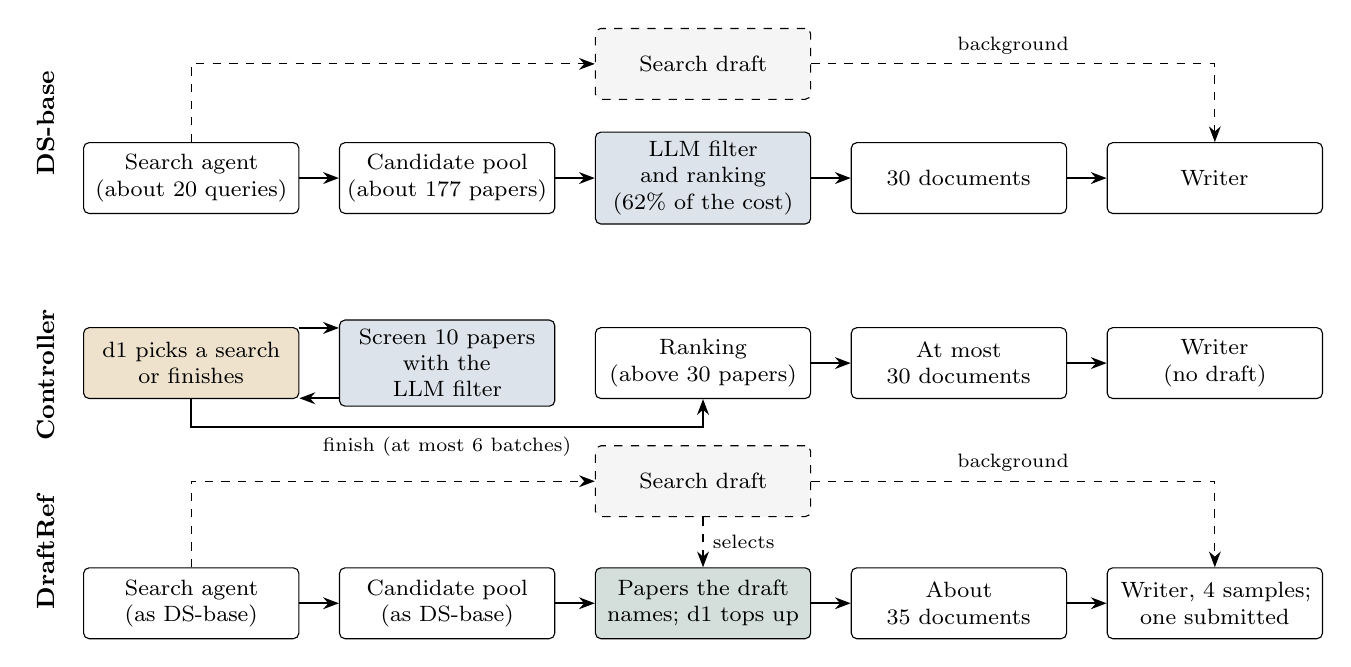
\begin{tikzpicture}[
  box/.style={draw, rounded corners=2pt, align=center, font=\footnotesize, minimum height=0.9cm,
    text width=2.5cm, fill=white},
  dbox/.style={box, dashed, fill=gray!8},
  lane/.style={font=\small\bfseries, rotate=90, anchor=center},
  arr/.style={-{Stealth[length=2mm]}, thick},
  darr/.style={-{Stealth[length=2mm]}, dashed}]
  % DS-base
  \node[lane] at (-1.85,0.7) {DS-base};
  \node[box] (a1) at (0,0) {Search agent\\(about 20 queries)};
  \node[box] (a2) at (3.25,0) {Candidate pool\\(about 177 papers)};
  \node[box, fill=cA!25] (a3) at (6.5,0) {LLM filter\\and ranking\\(62\% of the cost)};
  \node[box] (a4) at (9.75,0) {30 documents};
  \node[box] (a5) at (13.0,0) {Writer};
  \node[dbox] (ad) at (6.5,1.45) {Search draft};
  \foreach \i/\j in {a1/a2,a2/a3,a3/a4,a4/a5} \draw[arr] (\i) -- (\j);
  \draw[darr] (a1.north) |- (ad.west);
  \draw[darr] (ad.east) -| node[pos=0.25, above, font=\scriptsize] {background} (a5.north);
  % Controller
  \node[lane] at (-1.85,-2.5) {Controller};
  \node[box, fill=cB!30] (b1) at (0,-2.35) {d1 picks a search\\or finishes};
  \node[box, fill=cA!25] (b2) at (3.25,-2.35) {Screen 10 papers\\with the LLM filter};
  \node[box] (b3) at (6.5,-2.35) {Ranking\\(above 30 papers)};
  \node[box] (b4) at (9.75,-2.35) {At most\\30 documents};
  \node[box] (b5) at (13.0,-2.35) {Writer\\(no draft)};
  \draw[arr] (b1.18) -- (b2.162);
  \draw[arr] (b2.198) -- (b1.342);
  \draw[arr] (b1.south) -- ++(0,-0.35) -| node[pos=0.25, below, font=\scriptsize]
    {finish (at most 6 batches)} (b3.south);
  \draw[arr] (b3) -- (b4); \draw[arr] (b4) -- (b5);
  % DraftRef
  \node[lane] at (-1.85,-4.75) {DraftRef};
  \node[box] (c1) at (0,-5.4) {Search agent\\(as DS-base)};
  \node[box] (c2) at (3.25,-5.4) {Candidate pool\\(as DS-base)};
  \node[box, fill=cC!22] (c3) at (6.5,-5.4) {Papers the draft\\names; d1 tops up};
  \node[box] (c4) at (9.75,-5.4) {About\\35 documents};
  \node[box] (c5) at (13.0,-5.4) {Writer, 4 samples;\\one submitted};
  \node[dbox] (cd) at (6.5,-3.85) {Search draft};
  \foreach \i/\j in {c1/c2,c2/c3,c3/c4,c4/c5} \draw[arr] (\i) -- (\j);
  \draw[darr] (c1.north) |- (cd.west);
  \draw[darr] (cd) -- node[right, font=\scriptsize] {selects} (c3);
  \draw[darr] (cd.east) -| node[pos=0.25, above, font=\scriptsize] {background} (c5.north);
\end{tikzpicture}
\caption{The three pipelines. Shaded boxes are where they differ. DS-base screens its whole pool with
the executor; the controlled loop lets d1 decide how much to screen, and its writer gets no draft;
DraftRef keeps DS-base's search and draft, takes the writer's documents from the draft and replaces
the executor's filter with d1.}
\label{fig:pipelines}
\end{figure}

\paragraph{The loop.} The controlled loop (Figure~\ref{fig:pipelines}, middle) runs a task as a
sequence of retrieval decisions with up to four options. The abstract option screens the next ten
unseen papers of a BM25 search on the target abstract. This is a strong query: its top 150 hold 51 of
the 192 important citations on June development tasks, against 58 in DS-base's whole pool. The
explore option screens the first page of a keyword query that the executor proposes; the deepen
option screens the next page of the most productive keyword query; finish stops. Each option's
papers are fetched first, so the policy sees their titles, and the executor screens the chosen batch
with DS-base's own filter. A task screens at most six batches of ten, and hard rules keep enough
budget to write. On finish the relevant papers are ranked down to 30 if needed, and DS-base's
repaired writer writes from them. The loop has no search agent, so its writer gets no draft.

\paragraph{Policies.} d1 reads one multiple-choice question that describes the state (the task,
the budget left, the batches used, each search's yield and the latest relevant titles) and lists
the options with their costs and first titles. It finishes once the finish probability reaches 0.5
and otherwise takes the most probable search. The prompted executor answers the same question with
DeepSeek; it appears in the development comparisons only. The fixed rule alternates abstract and
keyword batches and finishes after three; a six-batch version matches d1's usual depth.

\paragraph{Training.} Decisions are rewarded without a judge, from the known important citations.
A step's retrieval return is $0.15\,\Delta R_e - 0.10\,\Delta C/B_0$, where the evidence recall
$R_e$ is the share of the task's important citations that the writer would receive if retrieval
stopped there; it mirrors the recall and cost terms of $U$. For the supervised warm start (d1-sft)
we take an early and a late decision point from each of untrained d1's training episodes, about 68
points in all, execute every legal option and continue each branch with d1 as deployed. With $G_a$
the return of option $a$'s branch and $G_{\text{best}}$ the best of them, the label is the soft
target $q(a) \propto \exp(-(G_{\text{best}} - G_a)/\tau)$ with $\tau = 0.005$, and a LoRA adapter
\cite{hu2022lora} is fit to it. For RL (d1-rl) we sample four trajectories from d1-sft at each of
eight late decision points and normalise each trajectory's return within its group, as in GRPO
\cite{shao2024deepseekmath}, with a clipped surrogate and a KL penalty to d1-sft. d1-rl is the last
update within a mean KL of 0.05 nats per decision. A trained model replaces d1 for the test only if,
on the nine validation tasks, it keeps d1's evidence recall, meets the depth thresholds and has no higher
regret, the best branch's return minus that of the option the model picks
(Appendix~\ref{app:training}).

\section{Results}
\label{sec:results}

\paragraph{Development.} On 20 June and 20 November development tasks the three controllers cost 12\%
to 28\% of DS-base, and their claim support is 0.08 to 0.13 higher on both sets. d1's nugget
coverage is 0.011 below DS-base's on November and 0.058 below on June (interval $-$0.118 to 0.001);
neither difference is resolved. d1 finds about as many important citations as DS-base, the fixed
rule fewer, and the prompted executor behaves like d1 (Appendix~\ref{app:dev}).

\paragraph{Training.} Neither trained model passes the gate: both finish after one batch on every
validation task. Their regret is lower than d1's (0.0034 against 0.0084), so by the training return
finishing early is nearly the best choice, yet it misses the important citations that later batches
find. Their evidence recall falls to 0.079 and 0.062, against d1's 0.174, so the test makes its main
claim with the untrained d1.

\begin{table}[t]
\centering\small
\begin{tabular}{llll}
\toprule
Measure & Required & d1 $-$ DS-base [95\% interval] & Holds\\
\midrule
Cost per task & upper bound $< 0$ & 28\% of DS-base (interval below 0) & yes\\
Nugget coverage & lower bound $> -0.02$ & \n.053 [\n.073, \n.033] & no\\
Citation precision & lower bound $> -0.05$ & +.129 [.109, .150] & yes\\
\midrule
Per-citation precision & lower bound $> -0.05$ & +.073 [.047, .098] & yes\\
Claim support & lower bound $> -0.05$ & +.122 [.106, .138] & yes\\
Reference recall (168 tasks) & lower bound $> -0.05$ & \n.031 [\n.062, .000] & no\\
\bottomrule
\end{tabular}
\caption{The registered main claim on the 180 held-out test tasks; it holds only if every bound
holds. Rows below the rule are our metrics. Reference recall is over the 168 tasks with important
citations.}
\label{tab:claim}
\end{table}

\paragraph{The held-out test.} Systems, adapters, task lists, sample counts and judges were frozen
before the first test call. The first 90 test tasks ran every arm and the other 90 ran DS-base and
d1, with two writer samples per task (one for closed-book): 1,890 reports, all completed.
Table~\ref{tab:claim} gives the main claim. d1 costs 28\% of DS-base and is better cited on all three
citation measures, but its nugget coverage is lower with the whole interval below zero, and its
reference recall misses the margin. The claim fails. The secondary claim for RL also fails: d1-rl's
$U$ is not above d1-sft's ($-$0.006, $p = .49$) and is below the three-batch fixed rule's ($-$0.042,
$p = .008$).

\begin{table}[t]
\centering\small
\begin{tabular}{l ccc V cccr}
\toprule
& \multicolumn{3}{c}{\emph{Benchmark metrics}} & \multicolumn{4}{c}{\emph{Our metrics}}\\
System & Nugget & Org.$^\dagger$ & Cite prec. & Ref.\ recall & Claim supp. & $U$ & Cost\\
\midrule
DS-base & \textbf{.420} & .678 & .387 & \textbf{.240} & .772 & .502 & 100\%\\
DS-base without its draft & .377 & .522 & .519 & .236 & .891 & .483 & 99\%\\
\midrule
Simple RAG & .357 & .344 & .470 & .093 & .830 & .499 & 2\%\\
Closed-book & .366 & .422 & .000 & .000 & .000 & .365 & 0.4\%\\
\midrule
Fixed rule, 3 batches & .362 & .464 & .582 & .176 & .871 & .524 & 11\%\\
Fixed rule, 6 batches & .356 & .469 & .512 & .212 & .884 & .506 & 27\%\\
d1 & .376 & .475 & .527 & .230 & \textbf{.898} & \textbf{.531} & 29\%\\
d1-sft & .333 & .333 & \textbf{.607} & .116 & .819 & .487 & 6\%\\
d1-rl & .329 & .342 & .605 & .104 & .809 & .482 & 5\%\\
\bottomrule
\end{tabular}
\caption{All arms on the first 90 test tasks. Cost is a percentage of DS-base's list cost; bold
marks the best value in a column. Reference recall leaves out the 7 tasks without important
citations, which $U$ counts as 0. $^\dagger$Reproduced poorly by our judge. The full table is in
Appendix~\ref{app:test}.}
\label{tab:arms}
\end{table}

Table~\ref{tab:arms} shows every arm on the first 90 tasks. Every arm covers fewer nuggets than
DS-base, and every such difference is resolved. d1 has the highest $U$, ahead of DS-base by 0.029
(interval 0.001 to 0.058) on these tasks but not on the other 90 (+0.008). d1-sft and d1-rl are the
cheapest controllers and the worst on coverage and recall. At the same six-batch limit and similar
cost, choosing searches with d1 instead of alternating them adds 0.020 nugget coverage and 0.018
reference recall on average, small next to the gap to DS-base.

\section{Why the controller falls short}
\label{sec:diagnosis}

Three observations point to what the writer receives rather than to the controller's retrieval
decisions. First, coverage depends little on retrieval at these levels. Closed-book, which retrieves and cites
nothing, covers 0.366 of the nuggets, inside the range of Simple RAG and the five controller arms
(0.329 to 0.376). The task's abstract alone covers 0.158, and the executor writes much of the rest
from what it already knows.

Second, removing DS-base's draft produces the controller's trade-off. Without its draft, DS-base
keeps its retrieval (reference recall $-$0.004) but loses 0.044 nugget coverage, as much as d1 loses
on the same 90 tasks. It also gains about as much citation reliability as d1: citation precision
+0.132 against d1's +0.140, and claim support +0.119 against +0.126. The draft adds about a tenth of
DS-base's nugget coverage and lowers its citation precision. The controlled loop has no draft and
shows the same trade-off. The comparison measures the draft's effect within DS-base rather than the
controller's retrieval, but the draft alone produces a gap of d1's size.

Third, the relevance filter loses important citations that the search had found.
Figure~\ref{fig:funnel} follows them through DS-base's pipeline on the 168 test tasks that have
them. Of 6.0 per task, 1.80 enter the candidate pool and the draft names 1.58 of these. The filter
drops 0.39 of the named ones and passes 1.32 important citations to the writer, which cites almost
all it receives. Keeping what the draft names would avoid that loss.

\begin{figure}[t]
\centering
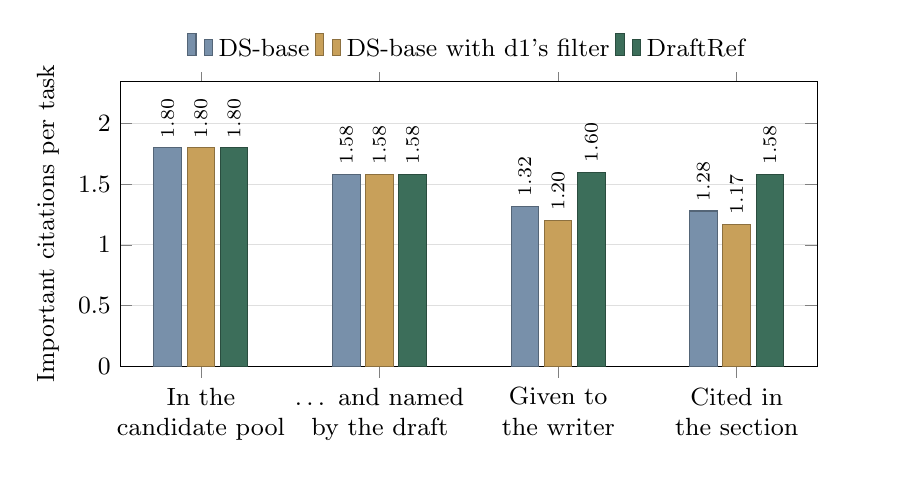
\begin{tikzpicture}
\begin{axis}[
  ybar, width=0.86\linewidth, height=5.2cm, bar width=10pt, ymin=0, ymax=2.35,
  ylabel={Important citations per task}, ylabel style={font=\small},
  symbolic x coords={pool,named,docs,cited},
  xticklabels={In the\\candidate pool, \ldots\ and named\\by the draft, Given to\\the writer,
    Cited in\\the section},
  xtick=data, x tick label style={font=\small, align=center, text width=3.2cm},
  enlarge x limits=0.15, tick label style={font=\small}, ytick={0,0.5,1,1.5,2},
  nodes near coords, every node near coord/.append style={font=\scriptsize, rotate=90, anchor=west,
    /pgf/number format/.cd, fixed, fixed zerofill, precision=2},
  legend style={font=\small, at={(0.5,1.03)}, anchor=south, legend columns=3, draw=none},
  ymajorgrids, grid style={gray!25}]
\addplot[fill=cA, draw=cA!70!black] coordinates {(pool,1.80) (named,1.58) (docs,1.32) (cited,1.28)};
\addplot[fill=cB, draw=cB!70!black] coordinates {(pool,1.80) (named,1.58) (docs,1.20) (cited,1.17)};
\addplot[fill=cC, draw=cC!70!black] coordinates {(pool,1.80) (named,1.58) (docs,1.60) (cited,1.58)};
\legend{DS-base, DS-base with d1's filter, DraftRef}
\end{axis}
\end{tikzpicture}
\caption{Where the important citations go, per task, on the 168 test tasks that have them (6.0 per
task). The three systems share one search and one draft; they differ in how the writer's documents
are chosen. DraftRef takes the papers the draft names and so keeps nearly all of them.}
\label{fig:funnel}
\end{figure}

\section{DraftRef: writing from the draft's references}
\label{sec:draftref}

\paragraph{Design.} DraftRef keeps DS-base's search agent, draft and writer
(Figure~\ref{fig:pipelines}, bottom) but changes how the writer's documents are chosen and how its
output is sampled. The documents are all pool papers whose arXiv ids appear in the draft, in the
draft's order, about 35 per task against DS-base's 30. d1 replaces the executor's relevance filter:
it reads each pool paper once, and when the draft names fewer than 30 papers (43 of the 180 test
tasks) the papers it judges relevant fill the list, most probable first. d1 supplies 3.7\% of the
documents. The saving comes from removing the filter's roughly 460 executor calls per task. The
writer draws four samples, and a text-only rule submits the one that uses more of the abstract's
content words and leaves fewer long sentences uncited; all four writes are charged. The ablation,
DS-base with d1's filter, gives the writer up to 30 papers that d1 judges relevant, most probable
first, without the draft rule.

\paragraph{The citation rule.} Citation precision scores a sentence by the share of its citations
that support the whole sentence, so a sentence citing three papers, one of which supports it,
scores one third. DraftRef's writer copies such bundles from the draft: 29\% of its long sentences
cite three or more papers, against 17\% for DS-base. The citation rule replaces the instruction to
cite as many sources as possible. It asks the writer to cite every source at least once, to end a
sentence where its source changes and to split sentences that join points from different sources,
keeping each point with its citation. Several sources may share a sentence only if each supports
all of it (Appendix~\ref{app:draftref}). Everything else, including the documents of all 720 writer
samples, is DraftRef's.

\begin{table}[t]
\centering\small\setlength{\tabcolsep}{4pt}
\begin{tabular}{l ccc V cccr}
\toprule
& \multicolumn{3}{c}{\emph{Benchmark metrics}} & \multicolumn{4}{c}{\emph{Our metrics}}\\
System & Nugget & Org.$^\dagger$ & Cite prec. & Ref.\ recall & Per citation & Claim supp. & Cost\\
\midrule
DS-base (mean of 2) & .436 & .689 & .400 & .211 & .454 & .776 & 100\%\\
DS-base with d1's filter & .424 & -- & .438 & .191 & .474 & .790 & 41\%\\
DraftRef & .443 & .750 & .399 & .253 & .416 & .839 & 41\%\\
DraftRef with the citation rule & \textbf{.448} & .722 & \textbf{.712} & \textbf{.254} & \textbf{.773}
  & \textbf{.875} & 40\%\\
\bottomrule
\end{tabular}
\caption{DraftRef on all 180 test tasks. The d1-based systems submit the best of four writer samples.
Unlike Tables 1 and 2, reference recall counts 0 on the 12 tasks without important citations. The
ablation was not judged on organization. Best-of-four costs include all four writes.}
\label{tab:draftref}
\end{table}

\paragraph{Results.} The registered claim for DraftRef required lower cost and non-inferior nugget
coverage and reference recall at a 0.02 margin; it holds ($p = .0066$, the largest of its three
tests). DraftRef costs 41\% of DS-base (Table~\ref{tab:draftref}). Its nugget coverage is +0.007
(interval $-$0.013 to 0.027), within the margin but not an improvement. Its reference recall is
+0.042 (0.023 to 0.061) and its claim support +0.063 (0.050 to 0.076). Figure~\ref{fig:funnel}
shows where the recall comes from: DraftRef gives the writer 1.60 important citations per task
against DS-base's 1.32, and the gain sits in the 47 tasks where the draft named a paper that the
filter dropped. As a filter on its own, d1 keeps fewer important citations than the executor's
filter (reference recall $-$0.020); the draft rule more than makes up for it. DraftRef keeps the draft and stays within DS-base's coverage margin; its saving comes from replacing executor screening, not from better retrieval decisions.

DraftRef's submitted citation precision equals DS-base's, but with samples averaged it is 0.024
lower, because its sentences bundle more citations. Against DraftRef, with both submitting the best
of four, the citation rule raises citation precision by 0.313 (0.288 to 0.337), while nugget
coverage (+0.004) and reference recall (+0.001) stay within the 0.02 margin ($p = .0109$).
Citations per cited sentence fall from 2.39 to 1.34, and the mean precision of a cited sentence
rises from 0.517 to 0.843. Claim support, which also credits a neighbour's citations, rises far less
(+0.036). The rule adds no call, and organization falls by an unresolved 0.028.

\paragraph{Validity.} DraftRef and the citation rule were fixed on development tasks before their
tests, but the 180 test tasks had already been used by the main test and later comparisons, so
neither is an independent test and their $p$-values do not account for the reuse. DraftRef also
submits the best of four samples while DS-base is the mean of two. With samples averaged on both
sides, DraftRef's differences from DS-base are +0.004 in nugget coverage and +0.043 in reference
recall; selection mainly lifts citation precision (+0.023) and claim support (+0.012).

\paragraph{Transfer to DRB2.} On six DRB2 tasks, with arXiv and web search for every system, d1 costs
26\% of DS-base, and every interval for a difference in rubric score includes zero
(Appendix~\ref{app:benchmarks}). Six tasks show that the controller runs on broader research
requests, but they cannot rank the systems there.

\section{Related work}

\paragraph{Deep research agents.} Recent agents train one model to search and write end to end: DR
Tulu \cite{shao2026drtulu} with reinforcement learning on rubrics that evolve with the policy, Tongyi
DeepResearch \cite{tongyi2025deepresearch} for long-horizon information seeking, and Search-R1
\cite{jin2025searchr1} from outcome rewards. AgentCPM-Report \cite{li2026agentcpm} alternates
drafting and deepening, close in spirit to DS-base's draft, and planner-centric RL
\cite{hussain2026planner} trains a planner on explicit research plans. We keep the executor frozen
and train only a small decision model, which can then be compared directly with a fixed rule.

\paragraph{Scientific synthesis.} Our starting point is DeepScholar-Bench \cite{patel2025deepscholar}
and its reference pipeline, built on LOTUS semantic operators \cite{patel2024lotus}. ResearchQA
\cite{li2025researchqa} and DRB2 \cite{li2026drb2} score long-form answers and reports with rubrics.
OpenScholar \cite{asai2026openscholar} and PaperQA2 \cite{skarlinski2024paperqa2} answer scientific
questions over large paper collections, STORM \cite{shao2024storm} writes articles from outlines
built by simulated questioning, and CREW \cite{dang2026crew} learns related-work generation as
multi-agent reinforcement learning.

\paragraph{Decision models and adaptive retrieval.} SearchJev \cite{cao2026searchjev} uses a small
decision model to score a search agent's legal options in one pass while a large model plans and
writes. decider-2b \cite{mapika2026decider} and d1-3B \cite{liquidai2026d1} are models of this kind,
and HarnessMDP \cite{yi2026harnessmdp} learns offline to control the harness around a fixed LLM.
Adaptive retrieval decides when to retrieve: Self-RAG \cite{asai2024selfrag} with reflection tokens,
FLARE \cite{jiang2023flare} from low-confidence tokens and Adaptive-RAG \cite{jeong2024adaptiverag}
from predicted query complexity. Our controller decides how much to screen and from which search,
under an explicit cost.

\paragraph{Citations and judges.} ALCE \cite{gao2023alce} introduced automatic citation recall and
precision; our per-citation precision and claim support also check each claim against the sources
it cites. Strong LLM judges agree well with human ratings but show position, verbosity and
self-preference biases \cite{zheng2023judge, panickssery2024selfpref}.

\section{Discussion and conclusion}

The course asks which changes most improve the completeness and reliability of a research report.
The retrieval policies we tested saved cost but did not add completeness. A 3B decision model
choosing what to screen cut the cost to 28\% of DS-base and produced better-supported sections, but
it lost coverage, and training it on retrieval-only rewards taught it to stop too soon. The larger
gains came after retrieval. In evidence selection, keeping the papers that DS-base's own draft names
raised reference recall at 41\% of DS-base's cost while coverage stayed within the margin. In
synthesis, one instruction about where sentences end raised citation precision from 0.399 to 0.712.
No change we tested raised nugget coverage resolvably above DS-base's, and the search remains the
bottleneck: 70\% of the important citations never reach the candidate pool.

Evidence is abstracts only, from one arXiv index. There is one executor,
which may know some target papers from pre-training, and the judges share its model family, so a
shared bias cannot be ruled out. Training used 34 tasks and a reward that sees only retrieval. A
fresh release of DeepScholar-Bench would give DraftRef and the citation rule an independent test.

\begin{thebibliography}{99}\small\raggedright
\setlength{\itemsep}{1pt}
\bibitem{asai2024selfrag}
A. Asai et al. Self-RAG: Learning to Retrieve, Generate, and Critique through Self-Reflection. ICLR,
2024.
\bibitem{asai2026openscholar}
A. Asai et al. Synthesizing Scientific Literature with Retrieval-Augmented Language Models. Nature,
650:857--863, 2026.
\bibitem{cao2026searchjev}
C. Cao et al. SearchJev: A Calibrated System-1 Model for Search Agents. arXiv:2610.05107v2, 2026.
\bibitem{dang2026crew}
H.-D. Dang et al. Assembling the CREW: A Collaborative Multi-agent Reinforcement Learning Framework
for Automated Related Work Generation. arXiv:2609.15721v1, 2026.
\bibitem{deepseek2026v41flash}
DeepSeek-AI. DeepSeek-V4.1-Flash: Pushing the Limits of KV Cache Compression. arXiv:2609.19969v1,
2026.
\bibitem{gao2023alce}
T. Gao et al. Enabling Large Language Models to Generate Text with Citations. EMNLP, 2023.
\bibitem{hu2022lora}
E. J. Hu et al. LoRA: Low-Rank Adaptation of Large Language Models. ICLR, 2022.
\bibitem{hussain2026planner}
M. A. Hussain, X. Wu, and Y. Lu. Planner-Centric Reinforcement Learning for Deep Research with
Structure-Aware Reward. arXiv:2605.30824v1, 2026.
\bibitem{jeong2024adaptiverag}
S. Jeong et al. Adaptive-RAG: Learning to Adapt Retrieval-Augmented Large Language Models through
Question Complexity. NAACL, 2024.
\bibitem{jiang2023flare}
Z. Jiang et al. Active Retrieval Augmented Generation. EMNLP, 2023.
\bibitem{jin2025searchr1}
B. Jin et al. Search-R1: Training LLMs to Reason and Leverage Search Engines with Reinforcement
Learning. COLM, 2025.
\bibitem{li2026agentcpm}
Y. Li et al. AgentCPM-Report: Interleaving Drafting and Deepening for Open-Ended Deep Research.
arXiv:2602.06540v1, 2026.
\bibitem{li2026drb2}
R. Li et al. DeepResearch Bench II: Diagnosing Deep Research Agents via Rubrics from Expert Reports.
arXiv:2601.08536v3, 2026.
\bibitem{li2025researchqa}
Li S. Yifei et al. ResearchQA: Evaluating Scholarly Question Answering at Scale Across 75 Fields with
Survey-Mined Questions and Rubrics. arXiv:2509.00496v2, 2025.
\bibitem{liquidai2026d1}
Liquid AI. d1-3B. Hugging Face model card, 2026. \url{https://huggingface.co/LiquidAI/d1-3B}.
\bibitem{mapika2026decider}
Mapika. decider-2b. Hugging Face model card, 2026. \url{https://huggingface.co/Mapika/decider-2b}.
\bibitem{panickssery2024selfpref}
A. Panickssery, S. R. Bowman, and S. Feng. LLM Evaluators Recognize and Favor Their Own
Generations. NeurIPS, 2024.
\bibitem{patel2024lotus}
L. Patel et al. Semantic Operators: A Declarative Model for Rich, AI-based Data Processing.
arXiv:2407.11418v3, 2024.
\bibitem{patel2025deepscholar}
L. Patel et al. DeepScholar-Bench: A Live Benchmark and Automated Evaluation for Generative Research
Synthesis. arXiv:2508.20033v2, 2025.
\bibitem{robertson2009bm25}
S. Robertson and H. Zaragoza. The Probabilistic Relevance Framework: BM25 and Beyond. Foundations
and Trends in Information Retrieval, 3(4):333--389, 2009.
\bibitem{shao2024storm}
Y. Shao et al. Assisting in Writing Wikipedia-like Articles From Scratch with Large Language
Models. NAACL, 2024.
\bibitem{shao2026drtulu}
R. Shao et al. DR Tulu: Reinforcement Learning with Evolving Rubrics for Deep Research. ICML, 2026.
\bibitem{shao2024deepseekmath}
Z. Shao et al. DeepSeekMath: Pushing the Limits of Mathematical Reasoning in Open Language Models.
arXiv:2402.03300v3, 2024.
\bibitem{skarlinski2024paperqa2}
M. D. Skarlinski et al. Language Agents Achieve Superhuman Synthesis of Scientific Knowledge.
arXiv:2409.13740v2, 2024.
\bibitem{tongyi2025deepresearch}
Tongyi DeepResearch Team. Tongyi DeepResearch Technical Report. arXiv:2510.24701v3, 2025.
\bibitem{yi2026harnessmdp}
H. Yi and X. Song. HarnessMDP: Learning to Control LLM Agent Harnesses with Offline Reinforcement
Learning. arXiv:2607.05458v3, 2026.
\bibitem{zheng2023judge}
L. Zheng et al. Judging LLM-as-a-Judge with MT-Bench and Chatbot Arena. NeurIPS Datasets and
Benchmarks Track, 2023.
\end{thebibliography}

\clearpage
\appendix
\section*{Appendix}
\addcontentsline{toc}{section}{Appendix}
\renewcommand{\thesubsection}{\Alph{subsection}}

\subsection{Metrics}
\label{app:metrics}

\begin{table}[H]
\centering\footnotesize\setlength{\tabcolsep}{3pt}
\begin{tabularx}{\linewidth}{>{\raggedright}p{2.6cm} X X}
\toprule
Metric & What it measures & Problem in the released code and our version\\
\midrule
Nugget coverage & Share of the paper's own section's key points the report fully covers & None found;
the primary completeness measure\\
Organization & Pairwise judgment of the report's structure against the paper's section, in both
orders & No code defect found; our judge reproduces it poorly ($\kappa$ 0.48 on 36 items)\\
Citation precision (cite\_p) & Mean over long sentences (50 characters or more) of the share of a
sentence's citations that support it & Uncited sentences score 0 and a multi-citation sentence counts
once, while the paper defines precision per citation. We add per-citation precision: supported
verdicts over all verdicts\\
Reference coverage & Share of important citations matched by arXiv id or by a similar cited title & Matches titles at
similarity above 0.8, crediting wrong papers. Reference recall matches exact arXiv ids, and is
undefined without important citations\\
Claim coverage & Share of long sentences supported by their cited documents & Checks neighbouring
sentences against the claim's own citations and adds the target abstract to the evidence. Claim
support asks whether the sentence's own citations, then a neighbour's, support it, with cited
documents as the only evidence\\
$U$ & Registered utility for selection and training & $N + 0.15R + 0.10P + 0.10S - 0.10\,C/B_0$; a
task without a report scores $-1 - 0.10\,C/B_0$; undefined reference recall counts 0\\
Evidence recall $R_e$ & Share of the task's important citations that are among the writer's documents; needs no report
or judge & Used for the training reward and the validation gate\\
\bottomrule
\end{tabularx}
\caption{Metrics. ``Long sentences'' are those of at least 50 characters, the ones the benchmark
scores.}
\end{table}

Failed or missing reports score 0 on every judged metric. Paired differences use each system's score
per task (the mean of its writer samples, or the submitted sample where one is selected), then report the mean difference over tasks with a 95\% $t$-interval
and a two-sided sign-flip permutation $p$-value (exact for 16 tasks or fewer, otherwise 20,000
draws). One writer sample and one judgment vary with a standard deviation of 0.073 per task at
fixed evidence, most of it the writer's. On 20 development tasks only nugget differences of about
0.05 can be resolved; on 90 test tasks, about 0.02.

\subsection{Baseline repairs and reproduction}
\label{app:repairs}

\begin{table}[H]
\centering\footnotesize\setlength{\tabcolsep}{3pt}
\begin{tabular}{l ccccc V ccc}
\toprule
System (June dev) & Nugget & Org.$^\dagger$ & Ref.\ cov. & Cite prec. & Claim cov. & Ref.\ rec. & Per cit. &
Claim supp.\\
\midrule
Paper, Llama-4 (63 tasks) & .241 & .206 & .103 & .674 & .851 & -- & -- & --\\
Paper, GPT-4.1 (63 tasks) & .348 & .809 & .166 & .788 & .899 & -- & -- & --\\
DS-base as released & .259 & .450 & .097 & .178 & .248 & .084 & .356 & .300\\
+ merge repair & .279 & .700 & .239 & .287 & .513 & .235 & .358 & .619\\
+ citation repair & .267 & .650 & .244 & .417 & .699 & .246 & .475 & .787\\
Paper protocol & .219 & .400 & .115 & .176 & .335 & .121 & .220 & .354\\
Paper protocol + citation repair & .207 & .325 & .119 & .461 & .631 & .126 & .541 & .702\\
Simple RAG & .183 & .300 & .152 & .431 & .711 & .160 & .458 & .850\\
\bottomrule
\end{tabular}
\caption{DS-base before and after the repairs on 20 June development tasks, with the paper's
published numbers (OpenAI judges, 63 tasks; the paper's citation precision is per citation, ours per
sentence). The merge repair raises the median candidate pool from
10 to 148 papers and the median number of cited sources from 6 to 22.}
\end{table}

With search and screening replayed so that only the writer differs, the citation repair changes
nugget coverage by $-$0.012 ($-$0.055 to 0.031), citation precision by +0.130 (0.036 to 0.224) and
claim support by +0.168 (0.034 to 0.301). Further run-time adaptations route LOTUS's search calls
through one metered client with the access policy, escape braces in abstracts that crashed the
pipeline, seed the ranking and pass the intended 10,000-token output limit to every stage. Under the
paper's recursive protocol DeepSeek covers 0.219 (June) and 0.410 (November) of the nuggets, against
0.241 and 0.358 for the paper's Llama-4 models, 0.348 for GPT-4.1 and 0.479 for GPT-4.1 with o3.
DeepSeek's list prices and per-task cost are about a seventh of GPT-4.1's. The baseline is the
repaired agentic DS-base without its unscored stages; the repaired paper protocol is lower on nugget
coverage ($-$0.059, $-$0.115 to $-$0.003).

\paragraph{Judge validation.} Table~\ref{tab:judges} lists the agreement checks. A blind spot-check, in which
a second model labelled 180 judge decisions, agreed 80\% on citation precision and claim support items
(both $\kappa$ 0.60), 86--96\% on DRB2 rubric scores and 65\% exactly on ResearchQA labels. Every
cite\_p disagreement concerned a multi-citation sentence that the DeepSeek judge accepted on partial
support. On 12 DRB2 development tasks, our DRB2 judge scored seven commercial systems' published
reports; its ranking has Spearman $\rho$ 0.90 against the GPT-5.5 leaderboard over the five systems
on it.

\begin{table}[H]
\centering\footnotesize\setlength{\tabcolsep}{3pt}
\begin{tabular}{lll}
\toprule
Benchmark & Item $\kappa$ (items) & Paired differences\\
\midrule
DeepScholar-Bench & cite\_p 0.81 (217), claims 0.93 (145), organization$^\dagger$ 0.48 (36) & same sign\\
ResearchQA & 0.74 (786 rubric labels) & same sign\\
DRB2 & 0.83--0.90 (1,113 rubric items) & same sign\\
\bottomrule
\end{tabular}
\caption{DeepSeek judges against the official judges on 139 reports from Simple RAG, closed-book and
DS-base. The rule set before the check required $\kappa \ge 0.6$ and no reversed difference;
organization fails it.}
\label{tab:judges}
\end{table}

\subsection{The controller}
\label{app:controller}

The state d1 reads contains the task, the remaining budget and the cap, the batch
count (such as ``2 of 6''), each search's pages, new papers and relevant papers so far, the totals screened
and relevant, and the latest ten relevant titles. Each option names its action, its cost and the
first titles it would screen. A state longer than d1's validated length (7,552 tokens) is shown with
fewer titles, never without the budget or the batch count. The abstract search reads its ranked list
to depth 150, a keyword query is followed for at most three pages, and the writer receives at most
30 documents. Before the policy sees the options, hard rules remove any search that would leave too
little budget to write, exceed six batches or bring no paper that an earlier option does not bring.
They also keep finish unavailable until the first relevant paper is found while a search is still
possible. When one option is legal it is executed without asking the policy. On DRB2 the research
request replaces the abstract, and the first batch comes from one web search.

\subsection{Training and the validation gate}
\label{app:training}

\paragraph{Supervised warm start.} Labels come from untrained d1's own episodes on the 34 training
tasks, so the model learns from the states it visits; validation labels come from its validation
episodes. Branches stop once the writer's documents are chosen; they are never written or judged.
Reward weights and metric versions were frozen before any label. Training uses LoRA, AdamW at
learning rate $5\times10^{-5}$, one warm-up step, two epochs, seed 0 and gradient clipping at 1.0.
The order of options is shuffled. The checkpoint with the lowest deployed regret on the validation
points (the best branch's return minus that of the option d1 would pick) is kept. A sanity task
(a paper's primary arXiv category among four, 2,000 training examples) raised held-out accuracy from
0.785 to 0.890, which confirms that the training loop works.

\paragraph{Bounded RL.} The eight decision points (one per task, after three to five batches, with at
least two search options) were fixed before any rollout. A group whose returns span less than 0.001,
or that contains a failed trajectory, trains nothing; seven of the eight groups trained. Each update
recomputes every decision's distribution and checks it against the logged probabilities. AdamW runs
at a constant learning rate of $2\times10^{-5}$, two groups per step (one in the fourth). After the fourth step the mean
KL to d1-sft was 0.047 nats per decision. d1-rl's regret on the validation points equals d1-sft's.

\begin{table}[H]
\centering\footnotesize\setlength{\tabcolsep}{3pt}
\begin{tabular}{lcccc}
\toprule
& d1 & d1-sft & d1-rl & Required\\
\midrule
Evidence recall of the writer's documents & .174 & .079 & .062 & $\ge$ d1\\
Batches before finishing & up to 6 & 1 on every task & 1 on every task & mean $\ge 3$, each $\ge 2$\\
Regret on the validation points & .0084 & .0034 & .0034 & $\le$ d1\\
Passes & -- & no & no & \\
\bottomrule
\end{tabular}
\caption{The validation gate on nine June validation tasks, two writer samples each.}
\end{table}

\subsection{Development results}
\label{app:dev}

\begin{table}[H]
\centering\footnotesize\setlength{\tabcolsep}{3pt}
\begin{tabular}{l ccccc V cccc r}
\toprule
System & Nugget & Org.$^\dagger$ & Ref.\ cov. & Cite prec. & Claim cov. & Ref.\ rec. & Per cit. & Claim supp. &
$U$ & Cost\\
\midrule
\multicolumn{11}{l}{\emph{June development, 20 tasks}}\\
DS-base & .277 & .600 & .249 & .419 & .698 & .248 & .480 & .788 & .367 & 100\%\\
d1 & .219 & .425 & .240 & .543 & .785 & .246 & .566 & .883 & .379 & 26\%\\
Prompted executor & .220 & .350 & .238 & .592 & .790 & .243 & .611 & .880 & .386 & 25\%\\
Fixed rule & .209 & .350 & .208 & .596 & .732 & .212 & .696 & .872 & .378 & 12\%\\
Simple RAG & .185 & .250 & .152 & .455 & .720 & .160 & .497 & .844 & .337 & 2\%\\
\midrule
\multicolumn{11}{l}{\emph{November development, 20 tasks}}\\
DS-base & .403 & .887 & .268 & .373 & .697 & .261 & .408 & .785 & .490 & 100\%\\
d1 & .392 & .575 & .293 & .539 & .817 & .261 & .544 & .915 & .556 & 28\%\\
Prompted executor & .386 & .662 & .273 & .589 & .799 & .240 & .604 & .891 & .551 & 25\%\\
Fixed rule & .394 & .537 & .211 & .587 & .771 & .175 & .642 & .868 & .557 & 12\%\\
Simple RAG & .298 & .512 & .160 & .470 & .709 & .169 & .486 & .829 & .450 & 2\%\\
\bottomrule
\end{tabular}
\caption{Development results, two writer samples per task. Cost is a percentage of DS-base's list
cost.}
\end{table}

\begin{table}[H]
\centering\footnotesize\setlength{\tabcolsep}{3pt}
\begin{tabular}{l c V ccc}
\toprule
Difference from DS-base & Nugget & Ref.\ recall & Claim support & $U$\\
\midrule
\multicolumn{5}{l}{\emph{June}}\\
d1 & \n.058 [\n.118, .001] & \n.002 [\n.136, .132] & +.095 [.048, .143] &
+.012 [\n.052, .075]\\
Prompted executor & \n.057 [\n.108, \n.005] & \n.005 [\n.147, .137] & +.092
[.041, .144] & +.019 [\n.041, .078]\\
Fixed rule & \n.069 [\n.126, \n.011] & \n.036 [\n.181, .109] & +.085 [.045,
.125] & +.011 [\n.053, .075]\\
\midrule
\multicolumn{5}{l}{\emph{November}}\\
d1 & \n.011 [\n.104, .081] & \n.001 [\n.119, .118] & +.131 [.090, .171] &
+.066 [\n.032, .164]\\
Prompted executor & \n.018 [\n.117, .081] & \n.022 [\n.144, .100] & +.106
[.055, .158] & +.061 [\n.040, .162]\\
Fixed rule & \n.009 [\n.072, .054] & \n.087 [\n.192, .018] & +.083 [.041,
.125] & +.067 [\n.004, .138]\\
\bottomrule
\end{tabular}
\caption{Paired differences from DS-base on the development sets, with 95\% intervals.}
\end{table}

On both sets d1 uses all six batches on 19 of 20 tasks. Its two writer samples from the same
evidence can differ widely: on one November task they cover 0.45 and 0.09 of the nuggets.

\subsection{The held-out test in full}
\label{app:test}

\begin{table}[H]
\centering\footnotesize\setlength{\tabcolsep}{3pt}
\setlength{\tabcolsep}{4pt}
\begin{tabular}{l ccccc V cccc r}
\toprule
System & Nugget & Org.$^\dagger$ & Ref.\ cov. & cite\_p & Cl.\ cov. & Ref.\ rec. & Per cit. & Cl.\ supp. &
$U$ & \$/task\\
\midrule
DS-base & .420 & .678 & .232 & .387 & .673 & .240 & .442 & .772 & .502 & .183\\
DS-base, no draft & .377 & .522 & .228 & .519 & .811 & .236 & .496 & .891 & .483 & .182\\
Simple RAG & .357 & .344 & .089 & .470 & .710 & .093 & .516 & .830 & .499 & .003\\
Closed-book & .366 & .422 & .000 & .000 & .000 & .000 & .000 & .000 & .365 & .001\\
Fixed, 3 batches & .362 & .464 & .166 & .582 & .765 & .176 & .634 & .871 & .524 & .021\\
Fixed, 6 batches & .356 & .469 & .200 & .512 & .784 & .212 & .513 & .884 & .506 & .050\\
d1 & .376 & .475 & .217 & .527 & .802 & .230 & .518 & .898 & .531 & .052\\
d1-sft & .333 & .333 & .108 & .607 & .685 & .116 & .778 & .819 & .487 & .011\\
d1-rl & .329 & .342 & .096 & .605 & .671 & .104 & .786 & .809 & .482 & .009\\
\bottomrule
\end{tabular}
\caption{All arms on the first 90 test tasks, every metric, list cost in dollars per task.}
\end{table}

\begin{figure}[H]
\centering
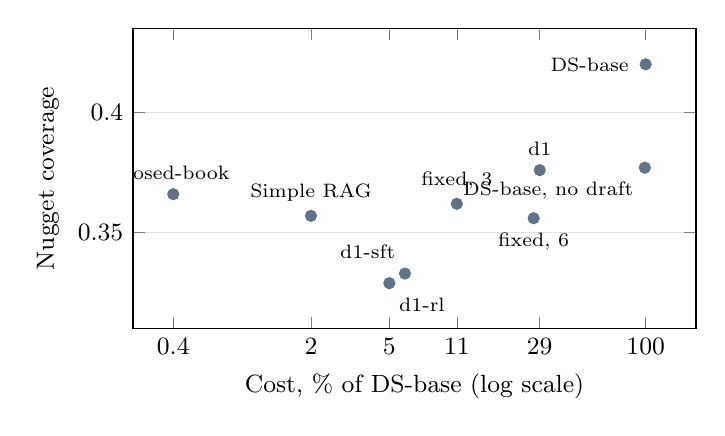
\begin{tikzpicture}
\begin{semilogxaxis}[width=0.72\linewidth, height=5.4cm, xlabel={Cost, \% of DS-base (log scale)},
  ylabel={Nugget coverage}, xmin=0.25, xmax=180, ymin=0.31, ymax=0.435, tick label style={font=\small},
  label style={font=\small}, ymajorgrids, grid style={gray!25},
  log ticks with fixed point, xtick={0.4,2,5,11,29,100}]
\addplot[only marks, mark=*, mark size=2pt, color=cA!80!black] coordinates {
  (100,0.420) (99,0.377) (2,0.357) (0.4,0.366) (11,0.362) (27,0.356) (29,0.376) (6,0.333) (5,0.329)};
\begin{scope}[font=\scriptsize]
\node[anchor=east] at (axis cs:92,0.420) {DS-base};
\node[anchor=north east] at (axis cs:97,0.375) {DS-base, no draft};
\node[anchor=south] at (axis cs:2,0.359) {Simple RAG};
\node[anchor=south] at (axis cs:0.4,0.368) {closed-book};
\node[anchor=south] at (axis cs:11,0.364) {fixed, 3};
\node[anchor=north] at (axis cs:27,0.354) {fixed, 6};
\node[anchor=south] at (axis cs:29,0.378) {d1};
\node[anchor=south east] at (axis cs:6,0.335) {d1-sft};
\node[anchor=north west] at (axis cs:5,0.327) {d1-rl};
\end{scope}
\end{semilogxaxis}
\end{tikzpicture}
\caption{Cost and nugget coverage of every arm on the first 90 test tasks.}
\end{figure}

Over all 180 tasks d1 costs 28\% of DS-base. The draft diagnostic on the first 90 tasks gives, for DS-base
without its draft against DS-base, reference recall $-$0.004 ($-$0.018 to 0.010) and nugget coverage
$-$0.044 ($-$0.075 to $-$0.012), against d1's $-$0.044 ($-$0.072 to $-$0.017). d1-rl's reference
recall against DS-base is $-$0.136 ($-$0.188 to $-$0.085).

\subsection{DraftRef in detail}
\label{app:draftref}

The search agent, which DraftRef replays from DS-base's cache, makes about 20 arXiv queries and reads
37 abstracts. Its draft names about 34 pool papers. DS-base's 30 documents hold 16 of them; DraftRef's
documents, about 35, are 96\% draft-named. The saving is DS-base's filter, about 62\% of its cost; d1
adds a nominal 1\% and the extra writes about 3\%, because writes after the first are mostly served
from the provider's prompt cache. The citation rule's recorded cost is slightly lower than DraftRef's
only because its first writes found DraftRef's prompts in that cache.

\begin{table}[H]
\centering\footnotesize\setlength{\tabcolsep}{3pt}
\begin{tabular}{l cc V cc}
\toprule
Difference [95\% interval] & Nugget & Cite prec. & Ref.\ recall & Claim support\\
\midrule
vs DS-base, as submitted & +.007 [\n.013, .027] & \n.001 [\n.018, .016] & +.042 [.023, .061] &
+.063 [.050, .076] \\
vs DS-base, samples averaged & +.004 [\n.012, .019] & \n.024 [\n.038, \n.009] & +.043 [.024,
.062] & +.051 [.039, .063] \\
vs DS-base with d1's filter & +.019 [\n.001, .039] & \n.038 [\n.059, \n.017] & +.062 [.039,
.085] & +.049 [.033, .065] \\
Rule vs DraftRef & +.004 [\n.015, .024] & +.313 [.288, .337] & +.001 [\n.001, .003] & +.036
[.026, .045] \\
Rule vs DS-base & +.012 [\n.003, .026] & -- & +.043 [.024, .062] & -- \\
\bottomrule
\end{tabular}
\caption{DraftRef's paired differences on the 180 test tasks (``vs'' rows are DraftRef minus the named system; ``rule'' is DraftRef with the citation rule). ``Samples averaged'' averages
DraftRef's four samples and DS-base's two, so neither side is selected.}
\end{table}

\begin{table}[H]
\centering\footnotesize\setlength{\tabcolsep}{3pt}
\begin{tabular}{lcccc}
\toprule
Per submitted section & DS-base & with d1's filter & DraftRef & with the citation rule\\
\midrule
Words & 426 & 449 & 457 & 503\\
Papers cited & 23.2 & 22.7 & 33.8 & 34.1\\
Long sentences with a citation & .71 & .76 & .77 & .84\\
Citations per cited sentence & 2.01 & 1.93 & 2.39 & 1.34\\
Long sentences with three or more citations & .17 & .17 & .29 & .06\\
Precision of a cited sentence & .560 & .577 & .517 & .843\\
Citation precision & .400 & .438 & .399 & .712\\
\bottomrule
\end{tabular}
\caption{How the sections cite, on the 180 test tasks.}
\end{table}

On other benchmark metrics DraftRef is higher than DS-base on organization (+0.061), claim coverage
(+0.072) and reference coverage (+0.044). The citation rule replaces the writer's instruction
``Cite as many sources as possible.'' with: ``Cite every source at least once, and end a sentence
where its source changes: do not join points from different sources in one sentence (with `and',
`while', a semicolon or a comma-separated list), even where the existing section content does; split
such sentences, keeping every point with its citation. Cite several sources in one sentence only if
each one supports the whole sentence.''

\subsection{DRB2 and ResearchQA}
\label{app:benchmarks}

\begin{table}[H]
\centering\footnotesize\setlength{\tabcolsep}{3pt}
\begin{tabular}{lccc}
\toprule
System & Total score & Difference from DS-base & Cost\\
\midrule
DS-base & .243 & -- & 100\%\\
Simple RAG & .274 & +.030 [\n.057, .118] & 7\%\\
Fixed rule & .221 & \n.022 [\n.105, .061] & 21\%\\
d1 & .197 & \n.046 [\n.142, .050] & 26\%\\
\bottomrule
\end{tabular}
\caption{Six DRB2 test tasks (three English, three Chinese), one writer sample each, arXiv plus at most
four web operations per task.}
\end{table}

\begin{table}[H]
\centering\footnotesize\setlength{\tabcolsep}{3pt}
\begin{tabular}{lccccc}
\toprule
Benchmark (metric, tasks) & Simple RAG & Closed-book & DS-base & DS-base $-$ Simple RAG\\
\midrule
DeepScholar (nugget coverage, 20) & .183 & .305 & .279 & +.096 [.034, .157]\\
ResearchQA (rubric coverage, 40) & .297 & .671 & .269 & \n.028 [\n.085, .030]\\
DRB2 (total, 12) & .297 & .428 & .255 & \n.042 [\n.198, .114]\\
\bottomrule
\end{tabular}
\caption{Baselines on the three benchmarks' development tasks, DS-base with the merge repair. On
ResearchQA DS-base produced nothing on 15 of 40 questions, where arXiv had no relevant paper.}
\end{table}

\subsection{Cost accounting and reproducibility}
\label{app:repro}

List cost prices every call at a frozen price book (DeepSeek-V4.1-Flash: \$0.30 per million
uncached input tokens, \$0.006 cached, \$1.20 output), including cached replays, and nominal tool
prices so that retrieval is never free (arXiv \$0.001 per call, web search \$0.008, d1 about
\$0.00014 per decision).

\begin{table}[H]
\centering\footnotesize\setlength{\tabcolsep}{3pt}
\begin{tabular}{lcc}
\toprule
List cost per task, June dev & DS-base & Controlled loop, d1\\
\midrule
Relevance screening & 167.3 calls, \$.0722 & 54.0 calls, \$.0238\\
Ranking & 251.3 calls, \$.0393 & 78.4 calls, \$.0114\\
arXiv searches and lookups & 19.3 + 36.9, \$.0562 & 8.6 + 0, \$.0086\\
Search agent or query proposals & \$.0081 & \$.0007\\
d1's decisions & -- & \$.0002\\
Writer & \$.0039 & \$.0031\\
Total & \$.180 & \$.048\\
\bottomrule
\end{tabular}
\caption{Where the money goes (one writer sample for d1).}
\end{table}

Every external dependency is pinned by commit or revision and checksum, and upstream code is patched
at run time, never edited. Executor calls are cached, so a rerun replays at no charge while keeping
its recorded list cost; judges are never cached. The repository (\repo) contains the code, the run
records behind every table and the commands to reproduce them; its README and \texttt{docs/} give
the details.

\end{document}
